\documentclass{article}
\RequirePackage[numbers,sort&compress,square,comma]{natbib}
\usepackage{graphicx}
\usepackage[a4paper, total={6in, 8in}]{geometry}
\bibliographystyle{IEEEtranN}
\begin{document}
\title{Machine Learning and Applications (MLAP) Open Assessment}
\author{Exam Number: Y0070813}
\date{\vspace{-5ex}}
\maketitle
%\tableofcontents
TODO - Check what happens if we take a log(0) - do we immediately quit or add 0 or something?
- Short circuit, data density	
 - 3.3.1 least squares error for finding weightings
- Laplacian eigenmaps needs to have the eigenvectors calculated for each unconnected sub-graph
\section{Task 1}
Code is given in \textit{FILENAME} and can be executed by running the following command: 


In the E-step I split each data-point into a set of configurations, one for every permutation of the hidden variables. I then calculate the Bayesian joint probability for each permutation, which acts as a weight in the M-step. This weight is normalised such that they sum to 1, providing a probability distribution for every combination in a data-row. 
In the M-Step I use this new dataset to count the number of times a variable is 1 given each of its parent states, this allows me to calculate the probabilities that are used in the E-step. For each variable in each data-point, I detect its parental state and increment the numerator or denominator depending on the variable state, the fraction is then evaluated to find the probability. 
To generate the log-likelihood I sum the log-likelihoods for each data-point, which is calculated by summing the likelihood for each permutation of the data-point's hidden variables, which is itself a product of the probability of each variable.
To detect the convergence of the algorithm I store the Log-likelihood for the previous iteration and compare it to the value calculated on the current iteration, if the difference is greater than 0.0001 then I report convergence.
\section{Task 2}
The adaptation of the code was achieved by writing a wrapper function \textit{FILENAME} to run the main code base with multiple initial starting values, additionally a parameter can be sent to the main file to allow the plotting of the log likelihood for each run. \\ 
The EM algorithm finds the local maximum for the Maximum Likelihood Estimator, therefore if there is a multi-modal distribution it is possible that the EM algorithm will not find the global maximum and instead one of many possible local maximums. Additionally, in the case of Bayesian Networks where the posterior probability is calculated from a combination of a prior distribution and a series of observations, if we ensure that there are no observations for a variable its posterior distribution will be based entirely on the prior distribution. To demonstrate this I have used the printer nightmare network again but by removing the observations for variable 1 and 3 I ensure that the posterior distribution, and therefore the parameters chosen by the EM algorithm, are only influenced by the prior distribution, in this case the initial values for the conditional probability. The network topography and dataset used are given in \textit{text} and \textit{text} respectively. \\
Using multiple different initial probabilities and comparing results, the values of 0.3 and 0.7 are chosen. These two initial values cause their variables parameter to be the initial value, and also have effect on child variables. This is shown in the table below. Additionally a plot of the log-likelihood against the EM iteration number is shown for both initial values.

\begin{center}
\begin{tabular}{|p{7cm}|p{7cm}|}
	\hline
	\begin{center}
		\textbf{Initial Probabilities of 0.3}
	\end{center}
	& 
	\begin{center}
		\textbf{Initial Probabilities of 0.7}
	\end{center}
	\\
	\hline
	\begin{verbatim}
	Convergence in 146 steps 
	Variable 0 has these parents ()
	P(0=1|() = 2.509891e-01 
	
	Variable 1 has these parents ()
	P(1=1|() = 3.000000e-01 
	
	Variable 2 has these parents ()
	P(2=1|() = 4.059554e-01 
	
	Variable 3 has these parents ()
	P(3=1|() = 3.000000e-01 
	
	Variable 4 has these parents ()
	P(4=1|() = 3.159885e-01 
	
	Variable 5 has these parents (0)
	P(5=1|('0')) = 0 
	P(5=1|('1')) = 9.828874e-01 
	
	Variable 6 has these parents (1, 2, 3)
	P(6=1|('0', '0', '0')) = 3.166248e-01 
	P(6=1|('0', '0', '1')) = 3.166248e-01 
	P(6=1|('0', '1', '0')) = 1.000000e+00 
	P(6=1|('0', '1', '1')) = 1.000000e+00 
	P(6=1|('1', '0', '0')) = 3.166248e-01 
	P(6=1|('1', '0', '1')) = 3.166248e-01 
	P(6=1|('1', '1', '0')) = 1.000000e+00 
	P(6=1|('1', '1', '1')) = 1.000000e+00 
	
	Variable 7 has these parents (0, 3)
	P(7=1|('0', '0')) = 2.754369e-01 
	P(7=1|('0', '1')) = 2.754369e-01 
	P(7=1|('1', '0')) = 6.529709e-01 
	P(7=1|('1', '1')) = 6.529709e-01 
	
	Variable 8 has these parents (3, 4)
	P(8=1|('0', '0')) = 1.862551e-01 
	P(8=1|('0', '1')) = 6.273635e-01 
	P(8=1|('1', '0')) = 1.862551e-01 
	P(8=1|('1', '1')) = 6.273635e-01 
	
	Variable 9 has these parents (0, 4)
	P(9=1|('0', '0')) = 4.993921e-01 
	P(9=1|('0', '1')) = 1 
	P(9=1|('1', '0')) = 3.910056e-01 
	P(9=1|('1', '1')) = 9.993642e-01\end{verbatim} & \begin{verbatim}
	Convergence in 64 steps 
	Variable 0 has these parents ()
	P(0=1|() = 4.393333e-01 
	
	Variable 1 has these parents ()
	P(1=1|() = 7.000000e-01 
	
	Variable 2 has these parents ()
	P(2=1|() = 4.059554e-01 
	
	Variable 3 has these parents ()
	P(3=1|() = 7.000000e-01 
	
	Variable 4 has these parents ()
	P(4=1|() = 3.058343e-01 
	
	Variable 5 has these parents (0)
	P(5=1|('0')) = 0 
	P(5=1|('1')) = 4.574197e-01 
	
	Variable 6 has these parents (1, 2, 3)
	P(6=1|('0', '0', '0')) = 3.166248e-01 
	P(6=1|('0', '0', '1')) = 3.166248e-01 
	P(6=1|('0', '1', '0')) = 1.000000e+00 
	P(6=1|('0', '1', '1')) = 1.000000e+00 
	P(6=1|('1', '0', '0')) = 3.166248e-01 
	P(6=1|('1', '0', '1')) = 3.166248e-01 
	P(6=1|('1', '1', '0')) = 1.000000e+00 
	P(6=1|('1', '1', '1')) = 1.000000e+00 
	
	Variable 7 has these parents (0, 3)
	P(7=1|('0', '0')) = 1.259833e-03 
	P(7=1|('0', '1')) = 1.259833e-03 
	P(7=1|('1', '0')) = 7.933800e-01 
	P(7=1|('1', '1')) = 7.933800e-01 
	
	Variable 8 has these parents (3, 4)
	P(8=1|('0', '0')) = 1.962714e-01 
	P(8=1|('0', '1')) = 6.262406e-01 
	P(8=1|('1', '0')) = 1.962714e-01 
	P(8=1|('1', '1')) = 6.262406e-01 
	
	Variable 9 has these parents (0, 4)
	P(9=1|('0', '0')) = 3.596072e-01 
	P(9=1|('0', '1')) = 1 
	P(9=1|('1', '0')) = 6.581454e-01 
	P(9=1|('1', '1')) = 1.000000e+00 
	\end{verbatim}\\ 
	\hline
\end{tabular} 
\end{center}

\begin{figure}[h!]
\centering
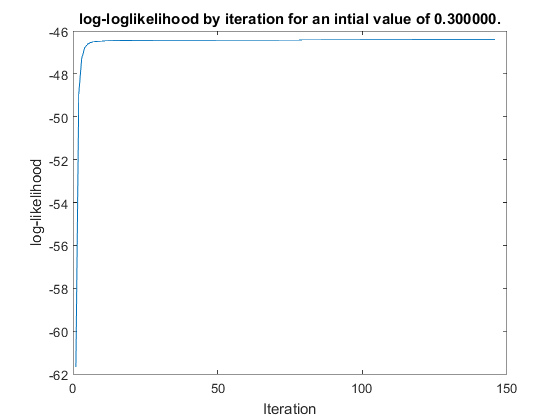
\includegraphics[width=0.7\linewidth]{images/LL3}
\label{fig:LL2}
\end{figure}
\begin{figure}[h!]
\centering
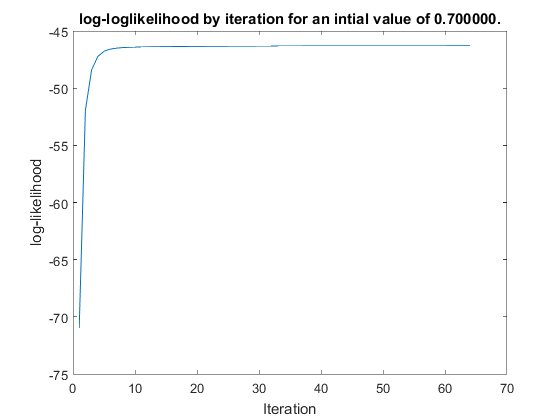
\includegraphics[width=0.7\linewidth]{images/LL7}
\label{fig:LL7}
\end{figure}
\textit{Graphs showing the log-likelihood against EM iteration number for initial values of 0.3 and 0.7, note the significantly larger number of iterations required to converge in the case of 0.3.}\\\\

Overcoming the dependence on initial values can be achieved either by using standard methods of minimising the risk of finding local maxima, such as simulated annealing or more simply random restart hill climbing. Ueda et al. developed a deterministic annealing algorithm for EM.\cite{ueda1998deterministic}

\section{Task 3}
\subsection{1. Qualitative Description of the algorithms}
\subsubsection{Locally Linear Embedding}
LLE first generates a list of neighbours for each data-point on the manifold. Then, using the assumption that the neighbourhood lies on a locally linear plane, a barycentric coordinate for each data-point as a series of weights for each of its neighbours such that the data-point can be re-constructed as a linear combination of its neighbours. These weights are then used in the lower dimensional space to re-construct the data-point. As each locally linear neighbourhood is overlapping, it is possible to re-construct the entire dataset in the low dimensional space. An error function is used for both the weight generation and point re-construction phases, to produce an optimal solution.
\subsubsection{Laplacian eigenmaps}
In this algorithm, we first generate a neighbourhood graph. Then a weight is applied to each edge, using one of two methods, either simply applying a weight of 1 for each edge (simple-minded) or by using a heat kernel. A Laplacian matrix is then generated from the weight matrix and its diagonal. By solving the generalized eigenvector problem for this Laplacian matrix and the weight matrix you find several solutions. These solutions are then ordered my ascending sizes of the eigenvalues. After removing the first eigenvalue, which will be zero, each of these solutions can be used as an embedding dimension for each data-point.
\subsubsection{Isomap}
Isomap can be thought of as an extension of Multi Dimensional Scaling, as it attempts to plot every data point in a lower dimensional space such that the high dimensional distances between data-points are maintained as best as possible. The distance metric is an estimate of geodesic distance between points over the manifold, generated by summing the euclidean distance between nodes on the shortest path between the nodes over a neighbourhood graph. Step 1 generates the neighbourhood graph, either with k-nearest neighbours or fixed radius, then the shortest paths between nodes are calculated and finally the estimated geodesic distance is used to apply MDS.
\subsection{2. Comparing the methods for embedding data into vector space}
The primary difference between the embeddings produced by ISOMAP in comparison to those generated by LLE and laplacian eigenmaps are the ability to represent the global structure of the data. As both LLE and LE are local techniques, the relationships between data points are only maintained over a local neighbourhood, with the global structure of the data potentially being warped or changed. On the other hand, ISOMAP ensures that the global structure of the data is concerved along with the local relationships. Therefore, on a global scale ISOMAP will produce a more truthful representation of the high dimensional data than LLE or LE. The main difference between LLE and LE is how truthfully the local distances are maintained through the transformation. In simple LE where the adjacency graph is populated by ones indicating a neighbourhood connection, there is no distance metric encoded at all. This means that if a point is close to another in high dimensional space then it will also be in low dimensional space, however the distances will not be maintained
ISOMAP PROS
preserves global structure
few free parameters
Guarantee of globally optimality
ISOMAP CONS
difficulties with holes in manifold
Sensitive to noise - short circuit 
Computationally intense due to dense matrix eigen reduction 
LLE PROS
No Local minima
one free parameter
simply linear algebra operations - so quick - eigenvectors from sparse matrices 
LLE CONS
can distort global structure 
***Seems to crush clusters into a single point?
Requires dense datapoints
LE PROS
Intrinsically emphasizes natural clusters 
stability due to intrinsic consideration of manifold structure
LE CONS
Has problems with non-uniform sampling?

local vs global methods
- Global gives more faithful representation of the global structure
- Local is more computationally efficient due to sparse matrix computations 
- Local may give useful results on a broader range of manifolds
http://papers.nips.cc/paper/2141-global-versus-local-methods-in-nonlinear-dimensionality-reduction.pdf
\subsection{3. Describing the methods mathematically}
\subsubsection{Locally Linear Embedding}
LLE begins by computing the neighbours for each data-point $x_i$ in $X = \{\vec{x}_1,...,\vec{x}_N\}$ either by placing a threshold on euclidean distance $\epsilon$, such that $x_j$ is a neighbour of $x_i$ if the euclidean distance in the high dimensional space $d_x(x_i,x_j) < \epsilon$. Alternatively, neighbours can be assigned based on $k$ nearest neighbours. We now need to compute the weights for each of the neighbours such that we can reconstruct the data-point as a linear combination of its neighbours. The following method is descried here.\cite{LLERoweis} First, we take the matrix $Z$, consisting of every neighbour of $x_i$ and subtract $x_i$ form every neighbour, we then compute the local co-variance of each element: $C = Z^TZ$. By solving $Cw = 1$ we find the weightings for each neighbour. We create an N by N matrix $W$ to store these weights, with $W_{ij}$ being 0 if $x_j$ is not a neighbour of $x_i$ and $\frac{w}{sum(w)}$ if they are neighbours.\\
We can now use this weight matrix to reconstruct $X$ in a lower dimensional space $d<<D$ with embedding $Y$. We do this by minimising the error function $\min_Y\sum\limits_{i}|Y_i-\sum\limits_{j}W_{ij}Y_j|^2$.\cite{ghodsi2006dimensionality} We can solve this error function by finding the eigenpairs for the matrix $M = (I-W)^T(I-W)$ and setting the rows of $Y$ to the ascending eigenvalues.
\subsubsection{Laplacian Eigenmaps}
The Laplacian Eigenmaps algorithm again starts by computing the nearest neighbours for every vector in $X = \{\vec{x}_1,...,\vec{x}_N\}$, either by using k-nearest neighbours or euclidean distance. This is stored as a graph, with an edge between each pair of data points which are neighbours. A weight is added to each edge, either simply 1 for each connection, creating an adjacency graph or by using a heat kernel function $W_{ij}=e^{-\frac{||X_i-x_k||^2}{t}}$. As t increases, the W value gets closer to the simple approach.\cite{hagueeigen} \\
We then compute the eigenpairs for the generalised eigen problem: $Lf = \lambda Df$ where D is a diagonal matrix formed by summing each row of W: ($D_{ii} = \sum\limits_jW_{ji}$) $L$ is the Laplacian matrix, which is calculated by $L = D-W$. By ordering the solutions to this formula, f, by the size of the associated eigenvalue and by removing the first f, which corresponds to an eigenvalue of 0 we can map the $X$ values to $Y$ values in m-dimensional space: $y_i = (f_1(x_i),...,f_m(x_i))$
\subsubsection{Isomap}
Starting with a set of $N$ data-points $X = \{\vec{x}_1,...,\vec{x}_N\}$ we first create a weighted graph, $G$, of the neighbourhood relations of X. For each data-point $x_i$ we calculate its neighbouring points $X_n = \{\vec{x}_1,...,\vec{x}_j\}$ either by placing a threshold on euclidean distance $\epsilon$, such that $x_j$ is a neighbour of $x_i$ if the euclidean distance in the high dimensional space $d_x(x_i,x_j) < \epsilon$. Alternatively, neighbours can be assigned based on $k$ nearest neighbours. An edge is then placed in $G$ between each data-point and its neighbours, with the edge weight being the euclidean distance between them. \\
Now we must generate a distance matrix $D_G$ of the geodesic distance between all points in $G$. We initialise this matrix by inserting the euclidean distance between points that are connected, $d_G(i,j) = d_x(i,j)$ if $i$ and $j$ are connected in the graph. If the points are not connected we need to estimate the geodesic distance between them by minimising the combined weights of the edges in the path between them over the graph. This is effectively finding the shortest path between every two points. In Isomap, this is achieved using the Floyd–Warshall algorithm.\cite{floyd1962algorithm} Thus $ d_G(i,j) = min\{d_G(i,j),d_G(i,k) + d_G(k,j)\}$ for all values of k. \\
Now that we have a pairwise geodesic distance matrix for $X$ we can apply the classic Multi Dimensional Scaling algorithm by calculating a kernel matrix, by double centring the distance matrix: $K = -\frac{1}{2}(I - \frac{J}{n})D_G(I-\frac{J}{n}))$ where J is an n-by-n matrix of 1's and I is the identity matrix. We then eigendecompose the kernel matrix $K = U\Lambda U^T$. After removing negative eigenvalues we then set $Y = \Lambda^{\frac{1}{2}}U^T$. The dimensionality of $Y$ is adjustable by removing eigenvalues and vectors from their respective matrices, in order of size.

All algorithms and formulas taken from \textit{'A Global Geometric Framework for Nonlinear Dimensionality Reduction'}\cite{tenenbaum2000global} except where cited.

\subsection{4. Description of a paper}
I chose \textit {'Wireless sensor networks localization with isomap'} by Wang et al,\cite{wang2009wireless} found by searching the list of articles citing the Isomap paper on Google Scholar, because of the novel use of Isomap, not so much for its properties as dimensionality reduction but because it uses geodesic distances for pairwise dissimilarity. The application is to estimate the locations of wireless sensors in a network based on the received signal strength between sensors, using MDS. As the data is error prone over long distances  Isomap is used as an extension. Additionally, they developed a centralised system, where isomap is better suited due to its global algorithm, LLE is used in decentralised applications.\cite{patwari2004manifold} The primary problem they encountered was setting the number of neighbours to choose for step 1 of Isomap, they overcame this by using an adaptive parameter selection method.
GRAPH REPRESENTATION?!
\bibliography{report}{}
\bibliographystyle{IEEEtranN}
\end{document}